\documentclass[12pt, twoside]{article}
\usepackage[letterpaper, margin=1in, headsep=0.5in]{geometry}
\usepackage[english]{babel}
\usepackage[utf8]{inputenc}
\usepackage{amsmath}
\usepackage{amsfonts}
\usepackage{amssymb}
\usepackage{tikz}
\usetikzlibrary{quotes, angles}
\usepackage{graphicx}
\usepackage{enumitem}
\usepackage{multicol}
\usepackage{hyperref}

\newif\ifmeta
\metatrue %print standards and topics tags

\title{IB Mathematics}
\author{Chris Huson}
\date{February 2022}

\usepackage{fancyhdr}
\pagestyle{fancy}
\fancyhf{}
\renewcommand{\headrulewidth}{0pt} % disable the underline of the header
\raggedbottom


\fancyhead[LE]{\thepage}
\fancyhead[RO]{\thepage \\ Name: \hspace{4cm} \,\\}
\fancyhead[LO]{BECA / IB Math 03-Quadratic functions\\* 9 February 2022}

\begin{document}

\subsubsection*{4.9 PreQuiz: Polynomial and rational functions}
\begin{enumerate}
\item The graph of a function $f$ is shown on the grid below.
    \begin{multicols}{2}
    \begin{enumerate}
      \item Write down $f(0)$
      \item Find $x$ for $f(x)=-3$.
      \vspace{0.25cm}
      \item Write down the domain.
      \item Write down the range. \vspace{1cm}
    \end{enumerate}
      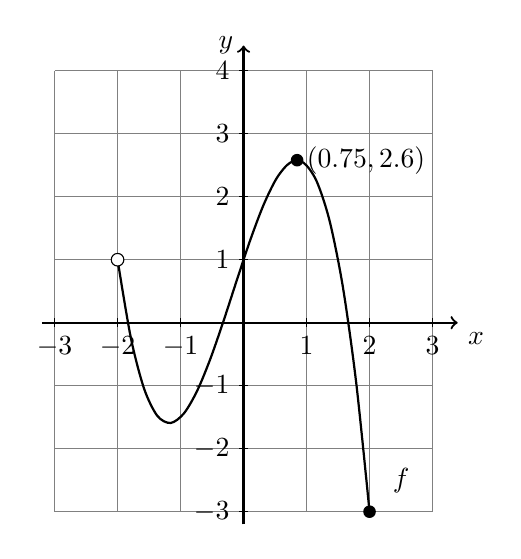
\begin{tikzpicture}[scale=0.8]
        \draw [help lines] (-3,-3) grid (3,4);
        \draw [thick, ->] (-3.2,0) -- (3.4,0) node [below right] {$x$};
        \draw [thick, ->] (0,-3.2)--(0,4.4) node [left] {$y$};
        \foreach \x in {-3,-2,-1,1,2, ...,3} \draw (\x cm,2pt)--(\x cm,-2pt) node[below] {$\x$};
        \foreach \y in {-3,-2,-1,1,2,3,4} \draw (2pt,\y cm)--(-2pt,\y cm) node[left] {$\y$};
        \draw [thick,smooth,samples=20,domain=-2:2] plot(\x,-\x^3-0.5*\x*\x+3*\x+1);
        \fill (2,-3) circle[radius=0.1];
        \fill (0.85,2.58) circle[radius=0.1] node [right]{$(0.75,2.6)$};
        \node at (2.5,-2.5){$f$};
        \fill [white] (-2,1) circle[radius=0.1];
        \draw (-2,1) circle[radius=0.1];
      \end{tikzpicture}
    \end{multicols}

\item Part of the function $f(x)=x^3-2x^2-5x+6$ is shown on the graph.
    \begin{center}
    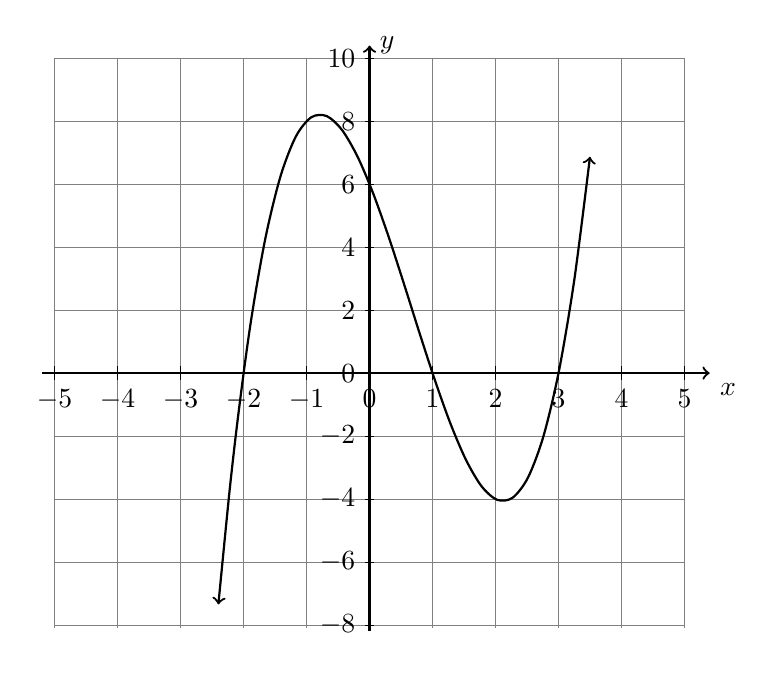
\begin{tikzpicture}[x=1cm, y=0.5cm, scale=0.8]
        \draw [help lines] (-5,-8.1) grid (5,10);
        \draw [thick, ->] (-5.2,0) -- (5.4,0) node [below right] {$x$};
        \draw [thick, ->] (0,-8.2)--(0,10.4) node [right] {$y$};
        \foreach \x in {-5,...,5}
            \draw[shift={(\x,0)}] (0,3pt)--(0,-3pt) node[below] {$\x$};
        \foreach \y in {-8,-6,...,10}
            \draw[shift={(0,\y)}] (2pt,0pt)--(-2pt,0pt) node[left]  {$\y$};
        \draw [<->,thick,smooth,domain=-2.4:3.5] plot(\x,{(\x)^3-2*(\x)^2-5*(\x)+6});
    \end{tikzpicture}
    \end{center}
    \begin{enumerate}
        \item Write down the $y$-intercept.
        \item Write down the $x$-intercepts.\vspace{0.5cm}
        \item Label the local maximum and local minimum as ordered pairs.
        \item Show that $1$ is an $x$-intercept because $x=1$ is a solution to $f(x)=0$.
    \end{enumerate}

\newpage
\item The rational function $\displaystyle f(x)=\frac{1}{x-2}+1$ and the linear function $\displaystyle g(x)=-\frac{3}{2}x+8$ are graphed below. 
    \begin{multicols}{2}
        \begin{enumerate}
            \item Find the solutions to $f(x)=g(x)$. \vspace{2cm}
            \item Write down the equation of the vertical asymptote to $f$.
        \end{enumerate} \vspace{0.5cm}
        \begin{flushright}
      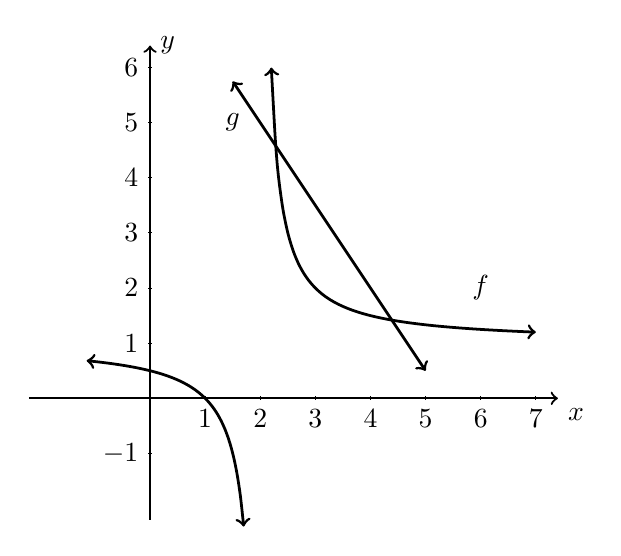
\begin{tikzpicture}[scale=0.7]
        %\draw [help lines] (-3,-3) grid (3,4);
        \draw [thick, ->] (-2.2,0) -- (7.4,0) node [below right] {$x$};
        \draw [thick, ->] (0,-2.2)--(0,6.4) node [right] {$y$};
        \foreach \x in {1,...,7} \draw (\x cm,1pt) -- (\x cm,-1pt) node[anchor=north] {$\x$};
        \foreach \y in {-1,1,2,...,6} \draw (1pt,\y cm) -- (-1pt,\y cm) node[left] {$\y$};
        %\clip (-2,-2) rectangle (6,7);
        \draw [<->,line width=1.0pt,smooth,samples=50,domain=2.2:7] plot(\x,{1/(\x-2)+1});
        \draw [<->,line width=1.0pt,smooth,samples=50,domain=-1.15:1.7] plot(\x,{1/(\x-2)+1});
        \draw [<->,line width=1.0pt,smooth,samples=20,domain=1.5:5] plot(\x,-1.5*\x+8);
        \node at (6,2){$f$};
        \node at (1.5,5){$g$};
      \end{tikzpicture}
    \end{flushright}
    \end{multicols}

\item Plot the function $h(x)=x^{3}+x^{2}-6x$, labeling the $x-$ and $y$-intercepts. Mark the local maximum and minimums as ordered pairs.
    \begin{center}
        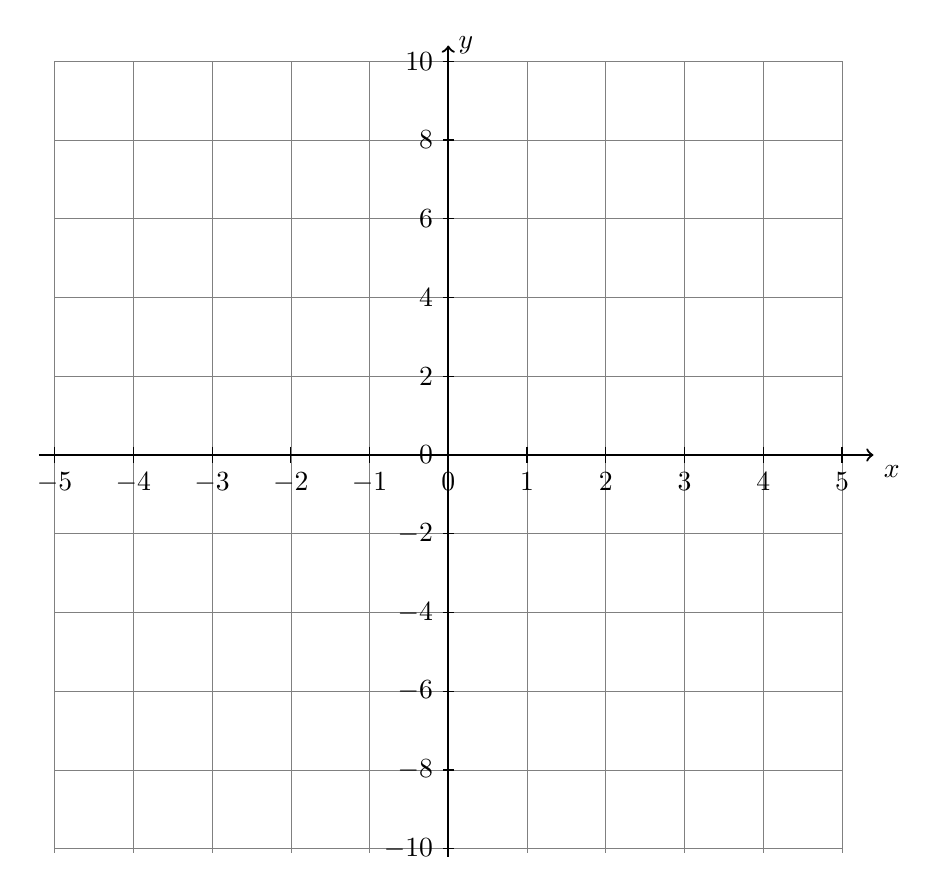
\begin{tikzpicture}[x=1cm, y=0.5cm]
            \draw [help lines] (-5,-10.1) grid (5,10);
            \draw [thick, ->] (-5.2,0) -- (5.4,0) node [below right] {$x$};
            \draw [thick, ->] (0,-10.2)--(0,10.4) node [right] {$y$};
            \foreach \x in {-5,...,5}
                \draw[shift={(\x,0)}] (0,3pt)--(0,-3pt) node[below] {$\x$};
            \foreach \y in {-10,-8,...,10}
                \draw[shift={(0,\y)}] (2pt,0pt)--(-2pt,0pt) node[left]  {$\y$};
            %\draw [<->,thick,smooth,domain=-3.5:2.5] plot(\x,{(\x)^3+(\x)^2-6*(\x)});
        \end{tikzpicture}
    \end{center}

\newpage
\item A cardboard box manufacturing company is building boxes with length represented by $x+1$, width by $5-x$, and height by $x-1$. The volume of the box is modeled by the function below.
    \begin{multicols}{2}
        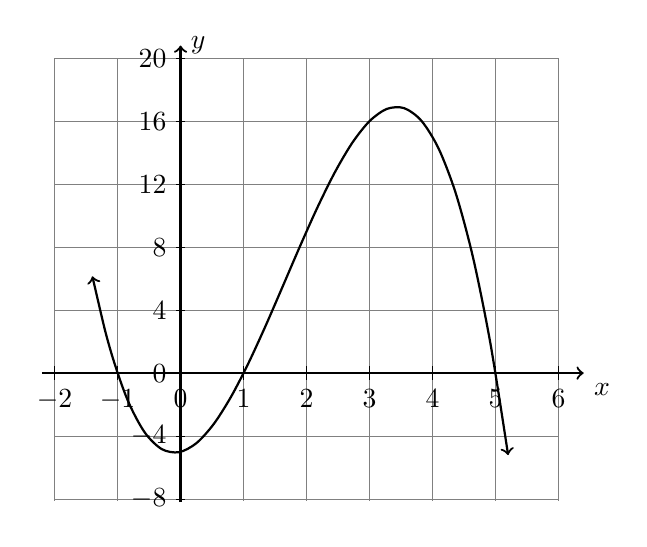
\begin{tikzpicture}[x=1cm, y=0.25cm, scale=0.8]
            \draw [help lines] (-2,-8.1) grid (6,20);
            \draw [thick, ->] (-2.2,0) -- (6.4,0) node [below right] {$x$};
            \draw [thick, ->] (0,-8.2)--(0,20.8) node [right] {$y$};
            \foreach \x in {-2,...,6}
                \draw[shift={(\x,0)}] (0,3pt)--(0,-3pt) node[below] {$\x$};
            \foreach \y in {-8,-4,...,20}
                \draw[shift={(0,\y)}] (2pt,0pt)--(-2pt,0pt) node[left]  {$\y$};
            \draw [<->,thick,smooth,domain=-1.4:5.2] plot(\x,{-(\x)^3+5*(\x)^2+(\x)-5});
        \end{tikzpicture}
    
    \begin{enumerate}[itemsep=0.75cm]
        \item Over what interval of positive $x$ values is the volume positive?
        \item Estimate the maximum possible volume of the box.
        \item Approximately the value of $x$ would maximize the volume of the box.
    \end{enumerate} 
\end{multicols}
%\vspace{0.5cm}

\item A function composed of four points $\{ (-1,4),(j,1),(4,3),(5,k) \}$ is plotted on the below.
    \begin{multicols}{2}
    \begin{enumerate}
      \item Write down $j$
      \item Write down $k$
      \item Write down the domain.\vspace{0.5cm}
      \item Add an ordered pair to the relation so that it would \emph{not} be a function.
    \end{enumerate}
      \begin{center}
      \begin{tikzpicture}[scale=0.8]
        %\draw [help lines] (-3,-2) grid (4,6);
        \draw [thick, ->] (-3.2,0) -- (5.4,0) node [below right] {$x$};
        \draw [thick, ->] (0,-0.5)--(0,5.4) node [left] {$y$};
        \foreach \x in {-2,-1,1,2,..., 5} \draw (\x cm,1pt) -- (\x cm,-1pt) node[anchor=north] {$\x$};
        \foreach \y in {1, 2, 3, 4, 5} \draw (1pt,\y cm) -- (-1pt,\y cm) node[anchor=east] {$\y$};
        %\draw [thick, <->] (-3.5,-1.5) -- (4.2,6.2);
        \fill (-1,4) circle[radius=0.1] node[above left]{$(-1,4)$};
        \fill (2,1) circle[radius=0.1] node[above]{$(j,1)$};
        \fill (4,3) circle[radius=0.1] node[above]{$(4,3)$};
        \fill (5,1) circle[radius=0.1] node[above right]{$(5,k)$};
      \end{tikzpicture}
      \end{center}
    \end{multicols}

\item Shown in the plot below is the function $f(x)=x^3+4x^2-1x-4$.
    \begin{enumerate}
        \item Write down the value of $f(0)$. On the graph, mark the point for $f(0)$ with a star.\vspace{0.75cm}
        \item Write down the solutions to $f(x)=0$. Mark them with ``X'' marks on the graph.\vspace{0.75cm}
        \item Mark the portion of the function that is \emph{decreasing} with a squiggly line.
    \end{enumerate}
    \begin{center}
        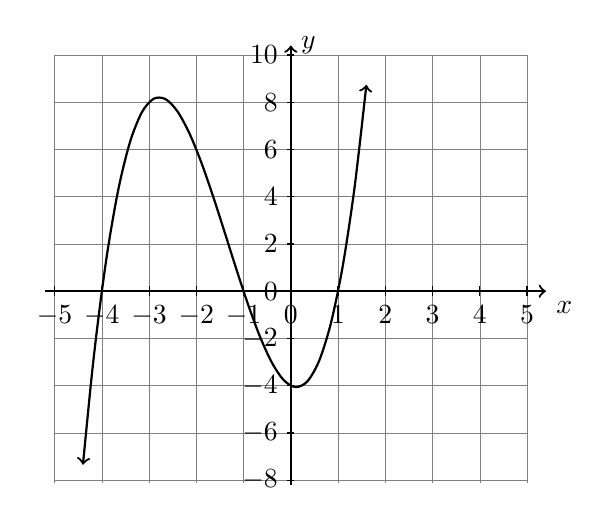
\begin{tikzpicture}[x=1cm, y=0.5cm, scale=0.6]
            \draw [help lines] (-5,-8.1) grid (5,10);
            \draw [thick, ->] (-5.2,0) -- (5.4,0) node [below right] {$x$};
            \draw [thick, ->] (0,-8.2)--(0,10.4) node [right] {$y$};
            \foreach \x in {-5,...,5}
                \draw[shift={(\x,0)}] (0,3pt)--(0,-3pt) node[below] {$\x$};
            \foreach \y in {-8,-6,...,10}
                \draw[shift={(0,\y)}] (2pt,0pt)--(-2pt,0pt) node[left]  {$\y$};
            \draw [<->,thick,smooth,domain=-4.4:1.6] plot(\x,{(\x)^3+4*(\x)^2-(\x)-4});
        \end{tikzpicture}
    \end{center}

\item The graph of a function $f$ is shown on the grid below.
    \begin{multicols}{2}
    \begin{enumerate}
      \item Write down $f(2)$
      %\vspace{0.25cm}
      \item Find $x$ for $f(x)=6$.
      \vspace{0.25cm}
      \item Write down the domain.
      \item Write down the range. \vspace{1cm}
    \end{enumerate}
      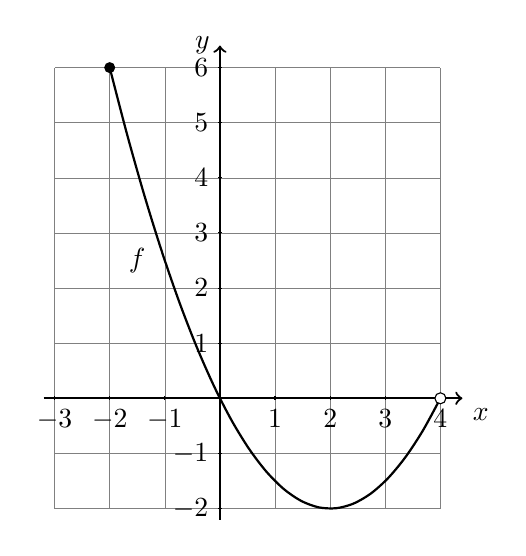
\begin{tikzpicture}[scale=0.7]
        \draw [help lines] (-3,-2) grid (4,6);
        \draw [thick, ->] (-3.2,0) -- (4.4,0) node [below right] {$x$};
        \draw [thick, ->] (0,-2.2)--(0,6.4) node [left] {$y$};
        \foreach \x in {-3,-2,-1,1,2, ..., 4} \draw (\x cm,1pt) -- (\x cm,-1pt) node[anchor=north] {$\x$};
        \foreach \y in {-2,-1,1,2,3,4,5,6} \draw (1pt,\y cm) -- (-1pt,\y cm) node[left] {$\y$};
        %\draw [thick] (-2,0) -- (0,4) -- (3,5);
        \draw [thick,smooth,samples=20,domain=-2:4] plot(\x,0.5*\x*\x-2*\x);
        \fill (-2,6) circle[radius=0.1];
        \node at (-1.5,2.5){$f$};
        \fill [white] (4,0) circle[radius=0.1];
        \draw (4,0) circle[radius=0.1];
      \end{tikzpicture}
    \end{multicols}
    \vspace{0.5cm}

\item The ramp in a skateboard park is modeled by the cubic function $h(x)=7.25-2.2x+0.011x^{3}$ where $h$ is the height in feet above ground and $x$ is the horizontal distance (ft).
    \begin{multicols}{2}
        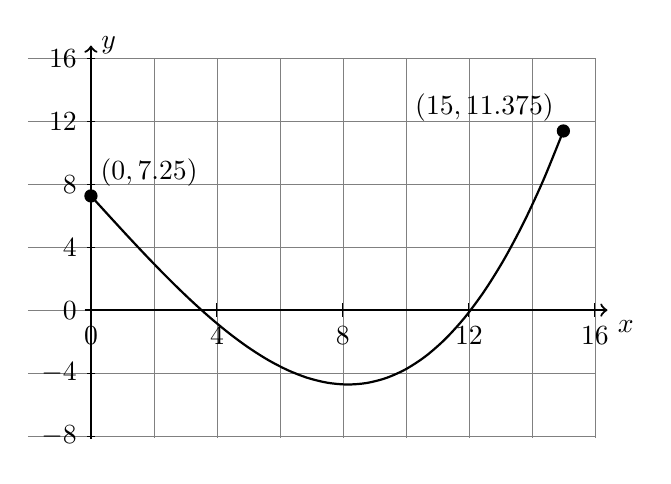
\begin{tikzpicture}[x=0.5cm, y=0.25cm, scale=0.8]
            \draw [help lines] (-2,-8.1) grid (16,16);
            \draw [thick, ->] (-0.2,0) -- (16.4,0) node [below right] {$x$};
            \draw [thick, ->] (0,-8.2)--(0,16.8) node [right] {$y$};
            \foreach \x in {0,4,...,16}
                \draw[shift={(\x,0)}] (0,3pt)--(0,-3pt) node[below] {$\x$};
            \foreach \y in {-8,-4,...,16}
                \draw[shift={(0,\y)}] (2pt,0pt)--(-2pt,0pt) node[left]  {$\y$};
            \draw [-,thick,smooth,domain=0:15] plot(\x,{0.011*(\x)^3+0*(\x)^2-2.2*(\x)+7.25});
            \fill (0,7.25) ellipse(3pt and 3pt) node [above right]{$(0,7.25)$};
            \fill (15,11.375) ellipse(3pt and 3pt) node [above left]{$(15,11.375)$};
        \end{tikzpicture}
    \begin{enumerate}[itemsep=0.75cm]
        \item How wide is the ramp in feet?
        \item Which lip is higher, the right or left lip? By how much?
        \item What is the maximum depth below ground of the ramp?
    \end{enumerate} 
    \end{multicols}
    
\item A rational function of the form $\displaystyle f(x)=\frac{1}{x+p}+q$ is shown on the grid below. 
    \begin{multicols}{2}
        \begin{enumerate}[itemsep=1cm]
            \item Write down the equation of the horizontal asymptote.
            \item  Write down the equation of the vertical asymptote.
            \item Hence, write down $p$ and $q$.
            \item Find $f(0)$.
            \item Solve for $x$ such that $f(x)=0$.
        \end{enumerate}
        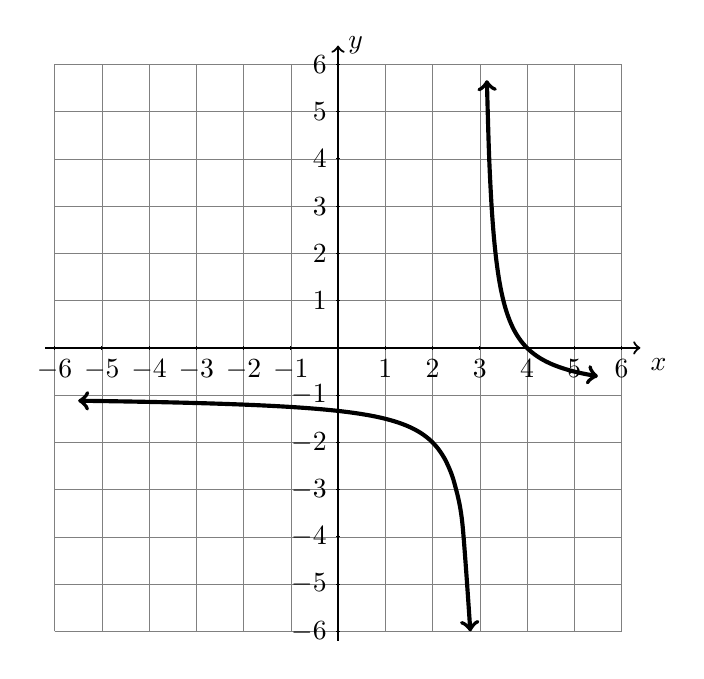
\begin{tikzpicture}[scale=0.6]
        \draw [help lines] (-6,-6) grid (6,6);
        \draw [thick, ->] (-6.2,0) -- (6.4,0) node [below right] {$x$};
        \draw [thick, ->] (0,-6.2)--(0,6.4) node [right] {$y$};
        \foreach \x in {-6,...,-3,-2,-1,1,2,...,6} \draw (\x cm,1pt) -- (\x cm,-1pt) node[anchor=north] {$\x$};
        \foreach \y in {-6,...,-3,-2,-1,1,2,...,6} \draw (1pt,\y cm) -- (-1pt,\y cm) node[left] {$\y$};
        \draw [<->,line width=1.5pt,smooth,samples=50,domain=-5.5:2.8] plot(\x,{1/(\x-3)-1});
        \draw [<->,line width=1.5pt,smooth,samples=50,domain=3.15:5.5] plot(\x,{1/(\x-3)-1});
        \end{tikzpicture}
    \end{multicols}

\item The temperature ($C^\circ$) over a 24 hour day starting at midnight is modeled by the function $f\left(t\right)=-0.0075t^{3}+0.17t^{2}+0.02t+5$.
    \begin{enumerate}[itemsep=1cm]
        \item Write down the temperature at midnight, when $t=0$.
        \item Over what interval is the temperature increasing?
        \item Find the maximum temperature during the day.  \vspace{1cm}
    \end{enumerate}
    \begin{center}
    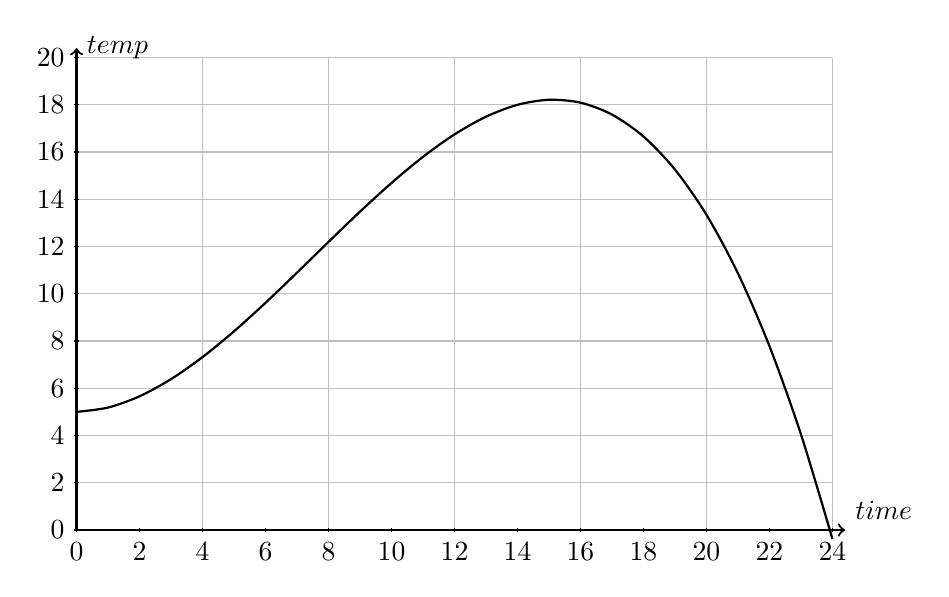
\begin{tikzpicture}[xscale=0.4, yscale=0.3]
        \draw [thin, color=lightgray, xstep=4.0cm,ystep=2.0cm] (0,0) grid (24,20);
        \foreach \x in {0,2,...,24}
        \draw (\x cm,3pt) -- (\x cm,-3pt) node[below] {$\x$};
        \foreach \y in {0,2,...,20}
        \draw[shift={(0,\y)},color=black] (2pt,0pt) -- (-2pt,0pt) node[left]  {$\y$};
        \draw [thick, ->] (0,0) -- (+24.4,0) node [above right] {$time$};
        \draw [thick, ->] (0,0) -- (0,20.4) node [right] {$temp$};
        \draw [thick, smooth,domain=0.:24] plot(\x,-0.0075*\x*\x*\x+0.17*\x*\x+0.02*\x+5);
    \end{tikzpicture}
    \end{center}

\end{enumerate}
\end{document}



